\documentclass[12pt,a4paper]{article}
\usepackage[utf8]{inputenc}
\usepackage{setspace}
\usepackage[german]{babel}
\usepackage{graphicx} 
\usepackage[T1]{fontenc}
\usepackage{amsmath}
\usepackage{amsfonts}
\usepackage{amssymb}
\usepackage{url}
\usepackage[bf]{caption}
\usepackage[a4paper]{geometry}
\usepackage{float}
\usepackage{acronym}
\usepackage{pdfpages}
\usepackage{enumitem}


\usepackage{jurabib}

\jurabibsetup{
	commabeforerest,
	ibidem=strict,
	%here you can change full citation, none, first
	citefull=first,
	see,
	titleformat={colonsep,all},
}

\renewcommand*{\jbauthorfont}{\textsc}
\renewcommand*{\biblnfont}{\scshape\textbf}
\renewcommand*{\bibfnfont}{\normalfont\textbf}
\AddTo\bibsgerman{%
	\renewcommand*{\ibidemname}{ebd.}
	\renewcommand*{\ibidemmidname}{ebd.}
}

\usepackage[bottom,hang]{footmisc}
\setlength{\footnotemargin}{0pt}


% Für source codes etc.
\usepackage{listings}

\usepackage{color}
\definecolor{gray}{rgb}{0.4,0.4,0.4}
\definecolor{darkblue}{rgb}{0.0,0.0,0.6}
\definecolor{cyan}{rgb}{0.0,0.6,0.6}

\lstset{
  numbers=left,   
  basicstyle=\ttfamily,
  columns=fullflexible,
  showstringspaces=false,
  commentstyle=\color{gray}\upshape
}

\lstdefinelanguage{XML}
{
  basicstyle=\footnotesize\ttfamily,
  morestring=[b]",
  morestring=[s]{>}{<},
  morecomment=[s]{<?}{?>},
  stringstyle=\color{black},
  identifierstyle=\color{darkblue},
  keywordstyle=\color{cyan},
  morekeywords={xmlns,version, type, about, resource, lang}
  % list your attributes here
}

\geometry{a4paper,left=25mm,right=25mm, top=25mm, bottom=25mm}
\onehalfspacing
\renewcommand{\familydefault}{ptm}

\usepackage[bottom,hang]{footmisc}
\usepackage{fnpct}


\setlength{\footnotemargin}{0pt}

\setlength{\parindent}{0pt}


\author{Christopher Pollin}
\title{\textbf{Formale, digitale Methoden und Modelle in den Geschichtswissenschaften. Am Beispiel digital edierter Rechnungsbücher}}
\date{\today{}, Graz}
\begin{document}
\pagenumbering{gobble}
\AdaptNoteOpt\footcite\multfootcite
\maketitle
\tableofcontents

\newpage
\pagenumbering{arabic}

\section{Einleitung}

Seit dem Zeitpunkt an dem es für Menschen den Bedarf gibt sich an Ereignisse oder Erkenntnisse, die für sie wichtig waren, zu erinnern, existieren auch Formen und Möglichkeiten Wissen darüber zu repräsentieren. Ein natürliches Beispiel dafür findet sich bereits in den ersten Hochkulturen als Menschen dokumentierte, dass jemand bei jemand anderen in der Schuld steht. Bereits um 3000 vor Christus lassen sich auf Tontafel Schuld und Kredit finden: "Alok schuldet dem Sumar 10 Eimer Korn". Wir können also feststellen, dass die Dokumentation ökonomischer Abhängigkeiten einer der ersten strukturierten Formen waren, um Wissen, wer wem etwas schuldet, festzuhalten und nieder zu schreiben.[ToDo Dan MCCreary] 
\\
Für Historiker*innen liefert uns diese Zeile einen Indiz auf ein Ereigniss in der Vergangenheit, das, wenn es in einen bestimmten historischen Kontext gestellt wird, für Forschungsfragen in den Geschichtswissenschaften relevant ist. Innerhalb der schriftlichen Überlieferung - der historischen Quelle - stecken semantische Strukturen, die dazu dienen können, ein Ereignis aus der Vergangenheit zu rekonstruieren. 
\\
Die Beschreibung der semantischen Struktur kann durch ein formales Modell erfolgen. Die Anwendung formaler Methoden unter Berücksichtigung eines solchen Modells kann als Grunlage dafür dienen Interpretationen der Vergangenheit - "wie es den gewesesen sein könnte" - mit einer gewissen Datengrundlage zu untermauern.
\\
Ziel dieser Arbeit soll eine theoretisch und praktische Auseinandersetzung mit den Herausforderungen und Möglichkeiten, die formalen, und somit auch digitale, Methoden und Modellen in der Geschichtswissenschaft mit sich bringen. Der praktische Anteil liegt dabei bei der Beschreibung der semantischen Anreicherung von digital edierten historischen Rechnungsbüchern in einem konkreten Projektkontext.
\\
\\
Am Anfang der Arbeit steht neben einer allgemeinen theoretischen Diskussion zur Verwednung empirischer, formaler Methoden in den Geschichtswissenschaften, in denen unter anderen Manfred THALLER\footcite{thaller2017digital}\footcite{thaller2017ungefahre} oder XXX viel beigetragen haben.
\\
Im zweiten Kapitel wird auf eine Technologie Stack, das Web of Data (aka Semantic Web) eingegangen, das die Grundlage zur formalen Beschreibung von INformation im World Wide Web liefert. Dafür ist eine konzeptionelle\footcite{berners2001semantic}\footcite{cardoso2007semantic} und technische\footcite{bernstein2016new} Erörterung dieses Themenbereiches notwendig. Ein notwendiger Schwerpunkt liegt dabei auf Wissensmodellierung\footcite{kelly2016practical} , Ontologien\footcite{stuckenschmidt2009ontologien} und \textit{Linked Open Data}\footcite{rietveld2015linked}\footcite{bauer2011linked} liegt, sowie einer kritischen Auseinandersetzung mit damit.\textit{Web of Data}\footcite{swartz2013aaron} Das Ontology Engineering\footcite{hitzler2016ontology} und das Reasoning\footcite{bursztyn2015reasoning} spielen dabei eine hervorgehobene Rolle.
\\
Das dritte Kapitel versteht sich als Quellenstudie und versucht den Quellentypus historischer Rechnungsbücher herauszuarbeiten. Dabei wird auf die Projektkontexte und Forschungsfragen im Kontext des Projektes DEPCHA eingegangen, eines durch die \textit{Andrew W. Mellon Foundation} geförderte und durch das \textit{Wheaton College Massachusetts} koordinierte Kooperation des Zentrums für Informationsmodellierung und Partnern aus den USA. Dieses Projekte verfolgt das Ziel semantisch angereicherte digitale Editionen von historischen Rechnungsbüchern, unter Verwendung von Web of Data Technologien, einem breiten Fachpublikum über das Web zugänglich zu machen.
\\
Darauf aufbauend wird die digitale Edition allgemein behandelt, und auf digitale Editionen historischer Rechnungsbüchern am Beispiel der angeführten Projektkontexte eingegangen. Der dabei verwendete Standard ist die Text Encoding Iniativ (TEI) auf dessen Grundlage die angeführten Editionen basieren. 
\\
Die digitale Edition in dieser Arbeit versteht sich als geschichtswissenschaftliche, quellenorientierte und inhaltsbezogene Edition, in der nicht jedes textuelel Phänomen ediert werden, muss, sondern die semantische Struktur der Quellen im Vordergrund stehen. Zur formalen Beschreibung semantischer Strukturen kann das \textit{Web of Data} herngezogen werden. Dies soll am Beispiel des DEPCHA Projektkontext und der Bookkeeping Ontologie, einem formalen Modell zur Beschreibung von Transaktionsprozessen in historischen Rechnugsunterlagen, durchgeführt werden.

\section{Formale Methoden und Modelle in den Geschichtswissenschaften}
Am ersten August des Jahres 1808 hat ein gewisser James Haley 1/4 viertel Pfund Pulver, 1 Pfund Kugeln und einen 1 Pfund Zucker zum Preis von 2 Schilling und 6 Pence im Laden der Stagville Plantage in North Carolina käuflich erworben. Solche Information über die Vergangenheit lassen sich in historischen Rechnungsbüchern finden. Dabei ist nicht der Einzeleintrag von großer Bedeutung für Fragestellungen in den Geschichtswissenschaften, sondern die Aggregation vieler Einzelinformationen, um eine Datengrundlage zu schaffen, auf der die weiter fachwissenschaftliche Arbeit der Historiker*innen ruht.
\\
\subsection{Theorien und Methoden der Geschichteswissenschaften}

''\textit{Die Historie ist eine Kunst, die auf Kenntnissen beruht, und weiter ist sie gar nichts'}'\footcite[TODO Seitenanzahl und .In][S.40--56]{mann1979pladoyer}
\\
Führte MANN im Jahr 1979 an, um auszudrücken, dass durch die Einführung neuartiger theoretischer Ansätze die Hauptaufgabe der Geschichtswissenschaften, das Erzählen von Geschichten, aufgeweicht wird. Diese neuartigen Ansätze etablierten sich ausgehend von Historikern wie Mommsen, Wehler oder Kocka in den 1960er Jahren, die ''\textit{eine Reform der Geschichtswissenschaft jenseits des Historismus}'' propagierten. Sie versuchten die Theorienbildung, wie in den systematischen Nachbardiszipilnen, wie etwa der Soziologie, in der Geschichteswissenschaften zu etablieren.
\\
''\textit{Erzählende Geschichte bedarf heute einer Theorie der Erzählung}'' beschreibt SOKOLL die heutige Situation, in der historische Forschung ohne theoretische Fragestellung nicht mehr möglicht ist. Methoden hingegen sind und waren ein stets anerkanntes Werkzeug in den Geschichtswissenschaften. Ein Blick auf die Vielfalt historischer Hilfswissenschaften, die sich mit der Erschließung von bestimmten Quellentypen beschäftigt, zeigt dies. 
\\
Neben Methoden der Erschließung historischer Quellen in ihrer Materialisierung als historische Hilfswissenschaften ist die Quellenkritik immanente Methode der Geschichtswissenschaft. Die Quellenkritik entwickelte sich aus dem Dreischritt von Heuristik, Kritik und Interpretation. Historiker*innen formulieren eine Fragestellung. Diese Fragestellung ist das Ergebnis, das sich aus einem spezifischen Forschungsstand und dem eigenen Erkentniss- sowie Interessenshorizont bildet. Relevante Quellen werden gesammelt, erschlossen und einer kritischen Prüfung auf Vollständigkeit, Glaubwürdikeit und Echtheit unterzogen. Die Ergebnisse aus dem Quellenstudium werden mit den Erkenntnissen von Fachkollegen*innen verglichen und in übergeordnete Kontexte eingeordnet.
Für DROYSEN mündet die Reflexion auf die historische Methode somit gleichsam wie von selbst in eine Theorie der historischen Erkenntnis -- als Lehre des deutenden Verstehens -- der sogenannten Hermeneutik. Aus diesem Verständnis heraus erwuchs 'die' Theorie der Geschichtswissenschaft.
\\
In der Geschichtswissenschaft von heute gibt es eine Vielzahl von Methoden, deren Abgrenzung zu Theorien oft verschwimmen. Diskusranalyse oder Konfliktransformation etwa lassen sich sowohl als Theorie, also auch Methode verstehen. Desweiteren verschwimmt auch die Unterscheidung zwischen qualitativer, interpretierender und quantitativer Methode. Erstere getragen von einem hemeneutischen, zweitere von einem emprischen Verständnis. 
\footcite[Vgl, TODO][S. 1--5]{sokollgrundlagen}

\subsection{Die historische Entwicklung formaler Methoden: ''Traditionalisten'' vs. ''Quantifizierer'' }
In den 1980iger Jahren standen sich im methodischen Zugang zu historischen Quellen zwei Gruppen gegenüber, die sich als ''Traditionalisten'' und ''Quantifizierer'' festmachen lassen können. Im Gegensatz zu den ''Traditionalisten'', die einen hermeneutischen Zugang wählten, um historische Quellen zu verstehen, übernahmen die ''Quantifizierer'' formale Methoden, wie etwa statistische Verfahren, aus den Sozialwissenschaften, um sie auf Quellenkorpora anzuwenden und die daraus gewonnenen empirischen Fakten für die Interpretation zu nutzen.\footcite[][S.XX-XX]{jarausch1985quantitative} Ergebnis dieser Auseinandersetzung war es, dass bei der Anwendung formaler Methoden besonders auf die Nachvollziehbarkeit geachtet werden muss, damit nicht Dinge, die nicht empirisch beweisbar sind, auch nicht so missverstanden werden können. Aus diesem Grund muss die Quelle ohne jegliche Vorannahmen zur Verfügung gestellt werden und einsehbar sein und die angewandte formale Modell bzw. die formale Methode in ihrer Gänze offen gelegt werden. Bei Zweiterem aber handelt es sich generell, um den Kern der Geschichtswissenschaften: die Interpretationen der Vergangenheit. Diese Interpretation sollte für andere nachvollziehbar sein und wissenschaftlichen Kriterien standhalten. Es wird empfohlen die grundlegenden Annahmen und Definitionen, die in der Interpretation von Quellen verwendet werden in einer gemeinsamen \textit{knowledge domain}, wie Thaller es nannte, zu formalisieren.\footcite[][S.XX-XX]{thaller2017historical}
\\ 
Nach dem abebben der formalen Methoden erleben sie zur Zeit eine neue Hochblüte in form von digitalen Methoden. 
\\
\\
Zentrale Konzepte in diesem Zusammenhang sind das \textit{Web of Data} bzw. \textit{Semantic Web} und \textit{Linked Open Data}. Diese Technologien ermöglichen es formale Modelle in den Geisteswissenschaften mensch und maschinenlesbar zusammen mit den Daten nachvollziehbar und nutzbar zu machen. Diese Technologien erleichtern den Austausch formaler Modelle. Über das Web können sie so leichter verteilt und nachgenutzt werden.

\subsection{Modellbildung in den Geschichtswissenschaften}

''\textit{Im wissenschaftlichen wie außerwissenschaftlichen Sprachgebrauch hat gegenwärtig der Modellbegriff zunehmend Relevanz erlangt. Bei zahlreichen passenden -- leider auch unpassenden -- Gelegenheiten ist von ''Modellen'' die Rede.}''\footcite[][S.1]{stachowiak1973allgemeine}
\\
\\
Bereits 1973 beschreibt STACHOWIAK in seiner Einleitung seiner ausführlichen Abhandlung zur Allgemeinen Modelltheorie, die unscharfe Verwendung des Modellbegriffes. STRACHOWIAK ein Modell als ''\textit{Ein Modell ist eine verkürzte, zweckorientierte Abbildung von der Wirklichkeit}''.\footcite[][]{stachowiak1973allgemeine}

\subsubsection{Modellbegriff}

Auch KOBLER führt an, dass der Modellbegriff in fast jeder wissenschaftlichen Disziplin vorzufinden ist, wobei eine einheitliche Definition des Begtriffes nicht vorzufinden ist. Kritik richtet sich oft daran, dass zur Definition des Begriffes, Konzepte wie Abstraktion Entität System etc. verwendet werden, die wiederum terminologisch unterschiedlich verwendet werden.
Im deutschen Sprachgebrauch lässt sich eine Doppelbedeutung festmachen: als Abbild von etwas, sowie Vorbild für etwas (jemand steht Modell beim Malen).\footcite[][S.129]{stachowiak1973allgemeine} Die Notwendigkeit des ersten Bedeutung geht daraus hervor, dass die Erfahrung und das Verstehen der Welt komplex ist. In ihrer Gesamtheit übersteigen sie die kognitiven Fähigkeiten des Menschen, weswegen ein Bereich eingeschränkt werden muss. Gerade diese Fertigkeit der Abstraktion und Generalisierung von Abbildern der Realität (von Dingen in der Welt) stellt die Grundlage der menschlichen Kultur. Der Fokus in dieser Arbeit betrachtet nun nur externalsierte, niedergeschriebene Modelle, die sich theoretisch in Datenmodelle überführen lassen. 
\\
In den unterschiedliche Disziplinen haben Modelle eine abweichende Funktion. In den Ingenierwissenschaften steht ein Modell für ein formales Modell, das einen Sachverhalt beschreibt und erklärt. In den Wirtschaftswissenschaften sind Modelle oft beschreibender Funktion. In der Wissenschaftstheorie werden Theorien in Form von mathematoschen Modellen dargestellt. In der Wirtschaftsinformatik werden Modelle für vielfältige Aufgaben eingesetzt, es gibt unterscheidliche Modelltypen.\footcite[][S.41-44]{kobler2010qualitat}
Zusammenfassung Modell
\\
\\
Eine Klassifiaktion lässt sich im Grad der syntaktischen dun semantischen Präzisierung umsetzen. Unterscheiden kann man informelle Modelle ohne eindeutige Beschreibungssystax, wie etwa natürliche Sprachen, semiformale Modelle nmit definierter Syntax, aber weitgehend ohne smeantische Konstruktionsregeln, wie etwas ER oder UML Modelle, oder etwas formale Modelle, die neben der Syntax auch die Semantik ausreichend beschreiben, wie MOdelle auf Grundlage deskruiptiver Logiken, wie etwas OWL. Für formale Modelle lassen sich dann Algorithmen definieren , um das Modell zu prüfen. Der Mensch aber kann auch mit nicht formalen Modellen arbeiten, im Gegensatz zum Computer. Es stehen also stark sturkturierte, formalisierte Modelle, die algorithmisch genutz werden können, offenen Modellen gegenüber, in die sich ein Mensch hineindenken kann.
\\
Konzeptuelle (konzeptionelle, ist ein Synonym) Modelle (conceptual model) bzw. Infomrationsmodelle (information model) sind beispielsweise in der Wirtschaftsinfomratik von zentraler Bedeutung, da Sie als Schnittstelle zwischen Informatik und Wirtschaftsinformatik besonders gut geeignet sind. Ich denke man kann diese genauso auch auf die Digitalen Geisteswissenschaften ummünzen.\footcite[][S.44-47]{kobler2010qualitat}
\\
\\
huhu\footcite[Vgl][S.99-108]{jannidis2017digital} 
\\
\\
Unterschieden werden eine normative, deskriptive udn explorative Funktion eines Modells.
\\
Modellierungen geschieht auf mehreren Ebenen: als modellierte Instanz, das heißt es ist ein Datenabbild eines Gegenstandes oder Textes (Instanz). Datenmodell sind Ausdruck eines Musters, das auf mehrere Instanzen anwendbar ist. Sowie Metamodell, die ein Ausdruck eines Musters ist, das auf mehrere Datenmodelle anwendbar ist, darstellen.
\\
\\
Es gibt vier verschiedene Möglichkeiten, Metamodelle zu gestalten:
\\
\\
Das Entity-Relationship-Modell (ER) baut auf den drei Begriffe Entität, Attribut und Relationauf. Die Entitäten (alle möglichen Untersuchungsobjekte) haben Eigenschaften (“Attribute“) und stehen zu anderen Entitäten in Beziehung („Relation“) Für die Beziehungen spielen die Kardinalitäten/Multiplizitäten eine wichtige Rolle, das heißt, dass ein Objekt unterschiedlich viele Beziehungen haben kann. Die Umsetzung eines ER erfolgt in der Informatik normalierweise in Tabellen, in denen die Beziehungen durch Verweise ausgedrückt werden, und mehrfach vorkommende Daten verringert werden.
\\
\\
Das Graphenmodell baut nur auf zwei Begriffen auf, nämlich der Entity und der Property (Eigenschaft) Rollen; die Eigenschaft ist eine Referenz auf eine andere Entität. Also es geht um „Knoten“ und Verbindungen zwischen Knoten („Kanten“). Entitäten können literal (also eine Zahl oder ein Text) oder eine Ressource (abstrakter Bezeichner für eine Entität) sein. Solche „Graphen“ können sowohl gerichtet als auch ungerichtet sein.
\\
\\
Klassen abstrahieren Entitäten. Das bedeutet, dass jedes Mitglied einer Klasse mindestens eine gemeinsame Eigenschaft mit den anderen Mitgliedern einer Klasse besitzt. Ohne dieser Eigenschaft ist es kein Mitglied. Um das zu bestimmen, muss die Eigenschaft, welche eine Klasse ausmacht, immer genau definiert werden.
\\
\\
Man kann seine Objekte aber auch als Hierarchien modellieren, bei denen Objekte und Eigenschaften Teil eines anderen Objektes sind. Wenn man hier etwas löscht, dann werden auch alle Unterelemente gelöscht.

\subsubsection{Was ist Informationsmodellierung}

\subsubsection{System}

Der Begriff System bezeichnet einen explizit von seiner Umgebung abgegenzten Gedankenbereich. Ein System besteht dabei aus einer Menge von Elementen, die miteinadner in Beziehung stehen und über spezifische Eigenschaften verfügen. Ein Eelement ist dabei nicht weiter spezifiziert, es handelt sich nur um atomare Bestandteile innerhalb eines Systems. Ein Syste, hat zu einer bestimmten Zeitpunk einen bestimmten Systemzustand, bzw kann man auf Grund des Verhaltens eines Systems eine Änderung (interner externer Ereignisse) beschreiben. Systeme können aus Systemen bestehen.
\footcite[][S.52-53]{kobler2010qualitat}

\subsection{Forschungsdaten in den Geschichtswissen}

Unter Daten versteht man ganz allgemein Zeichen, die Informationen darstellen und dem Zweck der weiteren Verarbeitung dienen. Die Informatik fasst den Begriff noch etwas spezifischer und versteht darunter Informationseinheiten in einer formalisierten und damit maschinenlesbaren und -bearbeitbaren Form. Das heißt, Informationen werden durch Daten so repräsentiert, dass sie vom Computer automatisch verarbeitet werden können.
\\
Was diese Daten am Ende repräsentieren, ist für die Definition erst einmal egal, und eigentlich auch für den Computer. Oder, wie es die Informatiker immer wieder betonen: Egal, ob die Daten Bilder, Texte, Filme, Objektbeschreibungen oder was auch immer repräsentieren, am Ende sind alles Daten und können als solche verarbeitet werden.
\\
Nun soll es hier aber um Forschungsdaten gehen. Als Forschungsdaten wiederum werden allgemein alle Daten definiert, die während eines Forschungsprozesses entstehen oder sein Ergebnis sind. Doch, und das ist an dieser Stelle die Frage, lässt sich diese Definition denn so einfach auf den geschichtswissenschaftlichen Forschungsprozess übertragen?
\\
Tatsächlich scheint diese Definition stärker an Fächern orientiert, die auf Grundlage von Experimenten und der dabei gewonnenen Messdaten arbeiten. Historische Arbeiten jedoch beruhen vor allem auf einem hermeneutischen Prozess, der auf der Lektüre und Verarbeitung einer größeren Zahl von Texten, Bildern und anderen Quellen und Informationen aufbaut. Hier stehen vielmehr die Quellen selbst im Vordergrund als die an ihnen vollzogenen „Messungen“ und die sich daraus ergebenden “Messdaten” (die es natürlich auch gibt).
\\
Während der Tagung wurde deutlich, dass die Teilnehmer letztlich mit zwei unterschiedlichen Begriffen von „geschichtswissenschaftlichen Forschungsdaten“ operierten: einem engeren und einem weiteren Begriff. Während der engere Begriff tatsächlich nur Daten einbezog, die im konkreten Forschungsprozess der einzelnen Projekte entstehen, wie z.B. die Textannotationen oder Metadaten, schloss der weitere Begriff auch die dem historischen Forschungsprozess zugrundeliegenden Quellen als Ganzes mit ein – so wie sie von Bibliotheken, Archiven und Museen wissenschaftlich aufbereitet und damit der potentiellen Nutzung durch die Forschung zur Verfügung gestellt werden.
\\
Dieser breitere Begriff macht dabei zugleich die Komplexität der Diskussion um „historische Forschungsdaten“ deutlich. Denn die Feststellung, dass im Sinne eines funktionalen Quellenbegriffs letztlich alles, was über vergangene Kulturen und Gesellschaften Auskunft geben kann, zur Quelle werden kann, gilt schließlich auch für deren digitale Repräsentation. Damit kann letztlich auch jede digitale Repräsentation von Texten, Bildern und Objekten sowie ihrer Präsenz in Zeit und Raum zu einem Forschungsdatum werden. Mit dem Blick auf eine digital organisierte und kommunizierende Gesellschaft heißt das auch, dass am Ende jedes Byte zu einer historischen Quelle und damit zu einem Forschungsdatum werden kann. \footcite[Vgl.][]{hiltman2018forschungsdaten}

\subsection{Modelle in den Geschichtswissenschaften}

Das Ziel: Aus den vielen Fäden ein allgemeingültiges Modell für die Repräsentation historischer Informationen in der Informationstechnologie zu machen.”
\\
\\
What we need is a discussion of the communalities between the underlying in-
formation models and the identification of properties, for which clear conceptual
models can be devised. Such clear conceptual models are a prerequisite for tech-
nical solutions, which ultimately can enable the exchange of data across the dif-
ferent approaches. Such conceptual models, therefore, are what we need as
standards.
\\
Analyzing someone else’s dataset is difficult. In fact, it is so
difficult that it is often simpler and less costly to create one’s own dataset from
scratch rather than use one prepared by another researcher from the same
underlying documentary sources.
\\
Thaller sagt, dass viel gewi Projekte einfach nur für eine Fragestellung ein System gebaut haben. Es ist verdammt schwer, dei Daten aus einerm anderen Projekt herauszuholen, zu verstehen, zu nutzen. Die gleiceh Quelle kann für unterscheidliche Forscher, unterschiedlich interessant sein. Er hebt hervor, dass es nmotwendig ist, dass wir Standardisierungen auf Eben konzeptuineller Modelle durchführen. 
\\
The approach to
standardization proposed by the Text Encoding Initiative (TEI) and developed
elsewhere in this volume is I feel, prescriptive.
\\
A standard must accommodate
each of these very different aims, but at the same time facilitate automatic
conversion of data structured for very different uses. From this perspective,
standardization needs to be descriptive rather than prescriptive
\\
\footcite[][S.204]{thaller2017need}

\section{Web of Data (aka Semantic Web)}


Beim \textit{TED Talk} im Jahre 2009 fordert Tim Burners-Lee das Auditorium auf mit ihm gemeinsam die Worte zu rufen: ''\textit{Raw Data Now!}''.\footnote{BERNERS-LEE Tim: The Next Web, \url{https://www.ted.com/talks/tim_berners_lee_on_the_next_web?language=de}, 05.04.2019.} Die Vision von Burners-Lee, dem Erfinder des World Wide Web, ist das sogenannte \textit{Semantic Web}:
\\
\\
''\textit{The Semantic Web will bring structure to the meaningful content of Web pages, creating an environment where software agents roaming from page to page can readily carry out sophisticated tasks for users.}''\footcite[][S.3]{berners2001semantic}
\\
\\
 Im Gegensatz zum klassischen Web, das als ein Web von Dokumenten betrachtet werden kann, versucht das \textit{Web of Data} Daten aus unterschiedlichen Quellen zu integrieren und miteinander zu verknüpft. Daten sollen so vorliegen, dass nicht nur Menschen diese in neuen Kontexten nutzen können, sondern auch Softwareagenten. Maschinen sollen in der Lage sein selbtständig die Struktur von Daten ''verstehen'' zu können, um bestimmte Aufgaben umsetzen zu können. Dabei handelt es sich aber weder um Maschinen die selbstständig lernen, oder gar eine künstliche Intelligenz, sondern um formalisiertes, maschinenenlesbares Wissen. Der Wissensbegriff in diesem Zusammenhang entspringt einer informationswissenschaftlichen Perspektive wie bei WERSIG, KUHLEN oder FAUVR-BULLE.
\\
Um diese - noch nicht erreichte Vision - in die Tat umzusetzen, sofern es nicht durch das Maschine Learning Paradigma obsolet wird, bedarf es mehrere aufeinander aufbauender technischer Grundlagen, die sich im \textit{Semantic Web Stack} manifestieren. Auf dessen Basis, dargestellt in Abbildung \ref{web_stack}, soll in diesem Kapitel die grundlegenden Technologien und Standards des \textit{Web of Data} erörtert werden.
\begin{figure}[h]
  \centering
	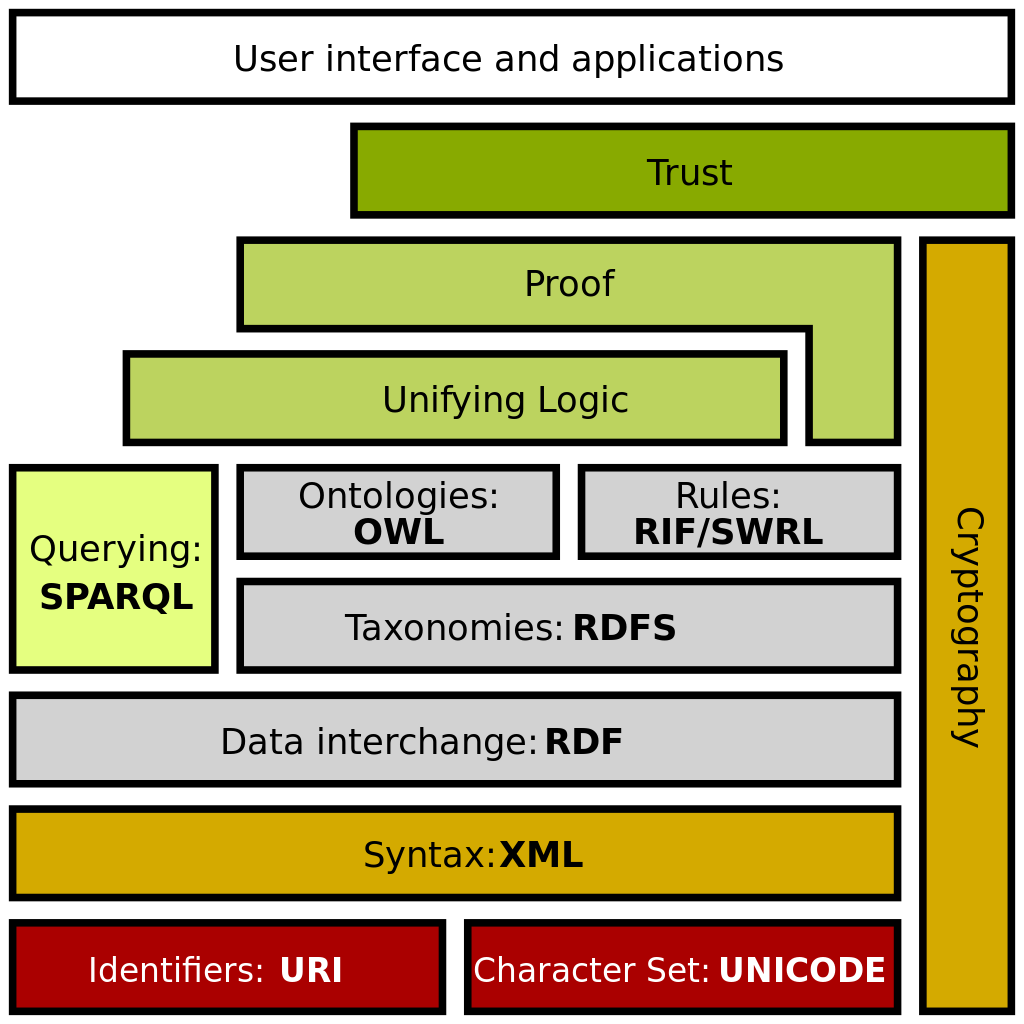
\includegraphics[width=0.65\textwidth]{img/web_stack.png}  
    \caption[Visualisierung eines Graphen auf Basis eines RDF-Datensatz, \protect\url{https://www.w3.org/TR/rdf11-primer/}, 10.04.2019.]{Visualisierung eines Graphen auf Basis eines RDF-Datensatz.}
  	\label{fig:web_stack}
\end{figure}

Das Semantic Web ist nicht erreicht. Zumindest nicht für die Allgemeinheit. Die großen Internetriesen hingegen everfügen über "ihre Semantic webs", in denen sie ihre eigeen Agenten mit ihrer großen Datenmenge arbeiten lassen.\footnote{\url{https://twobithistory.org/2018/05/27/semantic-web.html}}

\subsection{Resource Description Framework}

Das \textit{Resource Description Framework} (RDF) ist ein Datenmodell zur Darstellung und für den Austausch von Daten im Web. Daten werden in diesem Modell als Ressourcen definiert, wobei eine Ressource alles sein kann: ein Dokument, eine Person, ein physisches Objekt oder ein abstraktes Konzept. Über Ressourcen werden Statements der Form Subjekt-Prädikat-Objekt formuliert. Jedes Statement drückt eine Beziehung zwischen zwei Ressourcen aus. Das Subjekt und das Objekt stehen dabei für die beiden miteinander verbundenen Ressourcen; das Prädikat beschriebt die Art ihrer Beziehung. Diese Zusammensetzung von Subjekt, Prädikat und Objekt werden als Triples bezeichnet. Betrachtet man den Satz ''\textit{Bob ist befreundet mit Alice}'', dann lässt sich folgendes Triple extrahieren: \textit{<Bob>} als Subjekt, \textit{<ist befreundet mit>} als Prädikat und \textit{<Alice>} als Objekt. Ob \textit{Alice} mit \textit{Bob} befreundet ist geht aus diesem Statement noch nicht hervor, da jeder Relation in RDF nur eine Richtung definiert.\footcite[Vgl.][S.16-21]{powers2003practical} In der graphischen Darstellung wird schnell klar, dass es sich beim RDF Datenmodell um einen gerichtete Graphen handelt, der aus Knoten (Subjekt und Objekt), sowie aus Kanten (Prädikat) besteht, wie Abbildung \ref{fig:triple} zeigt.
\begin{figure}[h]
  \centering
	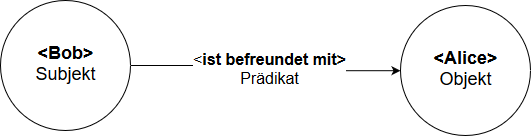
\includegraphics[width=0.75\textwidth]{img/triple.png}  
    \caption[ Semantic Web Stac]{ Semantic Web Stac}
  	\label{fig:triple}
\end{figure}

SCHREIBER und RAIMOND\footcite[Vgl.][]{schreiber2014rdf} erklären RDF in einem ausführlichen Beispiel an Hand folgenden Aussagen:
\\
\\
\textit{Bob ist eine Person.\\
Bob ist befreundet mit Alice.\\
Bob ist geboren am 4. Juli 1990. \\
Bob interessiert sich für die Mona Lisa.\\
Die Mona Lisa wurde von Leonardo da Vinci entworfen.}
\\
\\
Jede dieser Zeilen steht für ein Triple. \textit{Bob} ist Subjekt in vier der oben genannten Tripeln, \textit{Mona Lisa} tritt zweimal als Objekt und einmal als Subjekt auf. Dies ermöglicht es eine beliebige Menge an Triple zu einem komplexeren Graphen zusammenzusetzen und somit komplexere Sachverhalte beschreiben zu können. Abbildung \ref{fig:rdf_example} veranschaulicht das.
\begin{figure}[h]
  \centering
	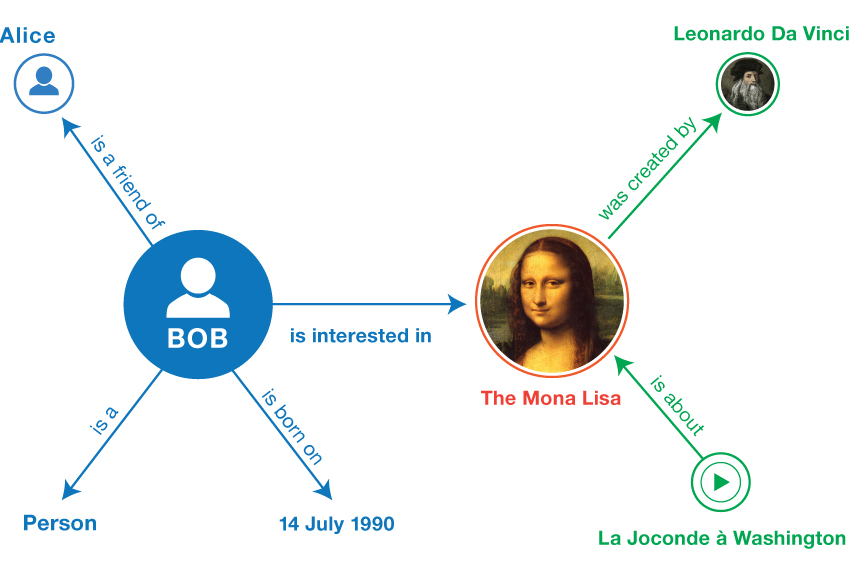
\includegraphics[width=1\textwidth]{img/rdf_example.png}  
    \caption[Visualisierung eines Graphen auf Basis eines RDF-Datensatz, \protect\url{https://www.w3.org/TR/rdf11-primer/}, 10.04.2019.]{Visualisierung eines Graphen auf Basis eines RDF-Datensatz.}
  	\label{fig:rdf_example}
\end{figure}

\textit{Uniform Resource Identifier} (URI) können in allen drei Positionen eines Triple erscheinen. Somit ist jeder Ressource, sowie jeder Beziehung zwischen Ressourcen durch eine URI identifizierbar. URI's sind durch ein erweiterbares Schema definiert, damit Ressourcen im Internet eindeutig adressiert werden können. Um dabei die Einheitlichkeit zu gewährleisten, folgen sie einem vordefinierten Satz von Syntaxregeln, der 5 Komponenten beinhaltet:\footcite[Vgl.][]{berners2004uniform}

\begin{center}
\textit{URI = scheme:[//authority]path[?query][\#fragment]}
\\
\end{center}


\begin{itemize}
\item \textbf{\textit{scheme}}: Definiert den Kontext und Typ. Bekannte Schemata sind beispielsweise die Webprotokolle \textit{Hyper Text Transfer Protocol} (http) oder das \textit{File Transfer Protocol} (ftp), sowie Notationskonzepte wie \textit{Uniform Resource Name} (URN)urn oder \textit{Digital Object Identifier} (doi).
\item \textbf{\textit{authority}}: Verwaltet Instanz in einem bestimmten vom Schema angegebenen Interpretationsraum, wie etwa das \textit{Domain Name System}.
\item \textbf{\textit{path}}: Der Pfad enthält – oft hierarchisch organisierte – Angaben, die zusammen mit dem Abfrageteil eine Ressource identifizieren. 
\item \textbf{\textit{query}}: Der Abfrageteil beinhaltet Daten zur Identifizierung von solchen Ressourcen, deren Ort durch die Pfadangabe allein nicht genau angegeben werden kann, wie beispielsweise ein Datensatz aus einer Datenbank, abgerufen werden
\item \textbf{\textit{fragment}}: Ist der optionale Fragmentbezeichner und referenziert eine Stelle innerhalb einer Ressource. Der Fragmentbezeichner bezieht sich immer nur auf den unmittelbar vorangehenden Teil des URI und wird von einem Hash (\#) eingeleitet.
\end{itemize}

Weiters werden URI in \textit{Uniform Resource Locator} (URL) und \textit{Uniform Resource Name} (URN) unterteilt. Wo URN Namen von Ressourcen eindeutig indetifuieren, wie etwa bei ISBN Nummern von Büchern, sind URL die gägnisten URI's, die den Ort einer Ressource addressieren und über einen Webbrowser auch aufrufen können.\footcite[Vgl.][S.21-22]{powers2003practical} Für das Triple \textit{<Bob>} \textit{<interessiert sich für>} \textit{<die Mona Lisa>} wird jeder Teilbestand eine URI und in der \textit{Turtle} Serialistion von RDF ergibt es folgenden Code:
\begin{lstlisting}[]
BASE   <http://example.org/>
PREFIX foaf: <http://xmlns.com/foaf/0.1/>
PREFIX xsd: <http://www.w3.org/2001/XMLSchema#>
PREFIX schema: <http://schema.org/>
PREFIX dcterms: <http://purl.org/dc/terms/>
PREFIX wd: <http://www.wikidata.org/entity/>

<bob#me> a foaf:Person ;
         foaf:knows <alice#me> ;
         schema:birthDate "1990-07-04"^^xsd:date ;
         foaf:topic_interest wd:Q12418 .
 
<wd:Q12418> dcterms:title "Mona Lisa" ;
            dcterms:creator <http://dbpedia.org/resource/Leonardo_da_Vinci> .
\end{lstlisting}


\subsection{Resource Description Framework Schema (RDFs)}

\subsection{Taxonomien: Simple Knowledge Organisation (SKOS)}

\subsection{Abfragesprache: SPARQL}

\subsection{Ontologien}


Informationsmodelle umfassen die Verwendung einer expliziten Sprache zur Informationsdarstellung.\footcite{kobler2010qualitat} 
\\
\\
Der Gegenstandsbereich der \textbf{Ontologie als Disziplin in der Philosophie} umfasst alles, das existiert. Das Erkenntnisziel, so MEIXNER, ist auf allgemeiner begrifflicher Ebene zu finden und beschäftigt sich mit der Einteilung des Seins und den Grundstrukturen der Wirklichkeit, sowie der Frage nach dem Wesen der Existenz. Die Ontologie verfolgt nicht das Ziel Erkenntnis über ein Objekt zu erhalten, es beispielsweise zu vermessen oder zu beschreiben, sondern stellt sich die Frage nach welchen allgemeinen Kriterien Objekte im Verhältnis zu ontologischen Begriffen wie Sein, Aktualität, Universalie, Exemplifikation, Sachverhalt oder Individuum stehen.\footcite{meixner1994wissenschaft}
\\
Der Begriff \textbf{Ontologie in der Informationswissenschaft bzw. Informatik} umfasst ein pragmatisches Konzept zum Austausch und zur Wiederverwendung von formalisierten und gemeinschaftlich verwendeten Wissensstrukturen durch ein gemeinsames Vokabular. Ziel dabei ist es Informationssysteme zu implementieren. Die Spezifikation eines solchen Vokabulars für eine bestimmte Domäne nennt man Ontologie.
\\
Der Begriff wird in zwei Disziplinen mit jeweils unterschiedlichen Fokus verwendet. Dennoch sehe ich Gemeinsamkeiten. Beide setzen sich mit der Frage auseinander, wie  die Welt sinnvoll strukturiert werden kann, damit wir uns besser darin zurecht finden können. In diesem Kapitel wird die informationswissenschaftlichen Dimension des Ontologie-Begriffs und seiner Nutzung in den digitalen Geisteswissenschaften diskutiert und der Frage nachgehen, ob Ontologien ein geeignetes Werkzeug zur Formalisierung von geschichtswissenschaftlichen Domänen darstellen. Dabei soll anfangs "Wissen" kurz aus informationswissenschaftlicher Sicht definiert werden und über das semantische Netz eine Brücke zur Ontologie geschlagen werden. 

\subsubsection{Vom Wissen, über das Semantische Netz zur Ontologie}
\textbf{Wissen} ist eine systeminterne Repräsentation vorliegender Erfahrungen eines Menschen zu einem bestimmten Zeitpunkt, die einem zu überprüfenden Anspruch auf Gültigkeit ausgesetzt sein muss. Als solches prägt Wissen das Handeln und Denken eines Menschen auf den unterschiedlichsten Ebenen und dient zur Lösung von Problemen. Das jeweils aktuelle Wissen bildet einen kontextuellen Rahmen, in dem ankommende und bestehende Information interpretiert und zu neuen Erfahrungen verarbeitet werden.\footcite{favre2001information}
\\
Diese Definition von Wissen -- eine stärker informationswissenschaftliche -- hat seinen, neben vielen Definitionen in anderen Fachbereichen, legitimen Ursprung.  Unterschiedlichen Disziplinen haben andere Fragestellungen und benötigen dafür ein anderes theoretisches Gerüst. Ein Wissensbegriff in der Philosophie, beispielsweise, sollte viel weiter gefasst sein, als ein Wissensbegriff in der Informationswissenschaft, dessen Aufgabe darin besteht als Hilfsmittel in der Entwicklung und Umsetzung von Informationssystemen zu fungieren. 
\\
\\
Mittels Ontologie lässt sich ''Wissen'' als Netzwerk beschreiben. Ein Netzwerk ist ein gerichteter Graph, bestehend aus einer Menge von Knoten und einer Menge von Kanten, die die einzelnen Knoten miteinander verknüpfen. Damit lassen sich (fast) beliebige Entitäten und deren Verknüpfungen miteinander abbilden. Die Überlegungen zu einem \textbf{semantischen Netz}, als gedanklichen Vorgänger der Ontologie, stammen von QUILIIAN, der damit ein formales Erklärungsmodell für '\textit{die menschliche Repräsentation von Wissen über Worte und ihre Bedeutung als Netzwerk von Begriffen und ihren Relationen}' \footcite{stuckenschmidt2009ontologien} beschreibt. Semantische Netze können einen Kompromiss zwischen menschenverständlicher Repräsentation einer Domäne  und der formalen Verarbeitbarkeit durch eine Maschine darstellen.\footcite{reichenberger2010grundlagen} Das ist dadurch gegeben, dass die Struktur des Graphen (=Netz), sich einfach in Rechnern als Matrizen abbilden lässt.
\\
Die Ontologie ist eine Erweiterung des semantischen Netzes und nach GRUBER kann sie durch ein \textbf{4-Tupel} definiert werden. C ist eine Menge von \textbf{Klassen} (concepts, classes - Mengen von Entitäten aus der Realität), R eine Menge von \textbf{Relationen} (properties - Beziehungen zwischen Klassen), I eine Menge von \textbf{Instanzen} (individuals - einzelne Entität aus einer Menge) und A eine Menge von \textbf{Axiomen} (axioms - logische Regel).\footcite{joostbreukera2009flood} C und R lassen sich dabei stets als Graph abbilden. Ein Beispiel zur Veranschaulichung: 
\\
Es existiert eine Klasse (C) "Katzen", die mit der Relation "ist ein" (R) mit einer Klasse "Säugetier" verbunden ist.  Die Individuals (I) "Garfield“ und "Tom" sind Instanzen der Klasse "Katzen" und erben alle Eigenschaften, die in der Klasse "Katzen" definiert wurden. Eine Regel kann definiert werden (A), sodass immer wenn eine Klasse eine "ist ein" Verbindung zu einer Klasse wie "Säugetier" hat, es ausgeschlossen ist, dass es eine zweite "ist ein"-Verbindung  gibt, die auf eine andere Klasse wie etwa "Vögel" referenziert. 
\\
\\
Der Begriff der Ontologie terminologisch unscharfe verwendet.\footcite[Vgl.][S.1]{gruber1993translation} Die Unterschiede sind klein, aber dennoch entscheidend und sollen im Folgenden diskutiert werden.
Eine der  ersten  Definitionen des Begriffs der Ontologie stammt von GRUBER: 
\begin{center}
 "\textit{An ontology is    an    explicit    specification    of    a conceptualization}
"\footcite[][S.69]{hoekstra2009ontology}
\end{center}
Eine "\textit{conceptualization}" beschreibt den Prozess einer Vereinfachung, aber Fokussierung, eines bestimmten Aspekts der Realität. 
So kann eine Ontologie als Dokumentation eines 
wissen- schaftlichen 
Prozesses agieren, in dem die Wirklichkeit abstrahiert und reduziert wird und gleichzeitig die Domäne bzw. Forschungsfrage hervorgehoben und amplifiziert wird.\footcite[Vgl.][]{thaller2017ungefahre}
Unter "\textit{explicit}" versteht man, dass die Bedeutungen aller von der Ontologie erfassten Begriffe klar und eindeutig definiert sein müssen. Dies beinhaltet alle ihre Eigenschaften, Beschränkungen und Beziehungen, innerhalb, als auch außerhalb der Domäne.\footcite{sure2003methodology}
BORST erweitert GRUBERS Definition um  '\textit{formal  specification  of  a shared  conceptualization}'.\footcite{borst1997construction}
"\textit{Formal}" ergänzt dabei die Definition um die Notwendigkeit, dass Ontologien maschinenlesbar sein müssen. Erst diese Eigenschaft hebt sie von anderen Methoden zur Formalisierung von konzeptionellen Datenmodellen hervor. Der Zusatz "\textit{shared}" reflektiert die Tatsache, dass eine Ontologie Wissen erfasst, das durch den Konsens einer Gruppe - z.B. durch einen wissenschaftlichen  Diskurs - akzeptiert wird. Eine Ontologie darf nicht im Stillen von einer Person alleine entwickelt werden, sondern sollte in einem iterativen Prozess (Ontology Engineering) des Austausches und der Diskussion mit anderen entstehen. Ein solcher Prozess kann wie folgt ablaufen:
\begin{itemize}
\item Definition der Notwendigkeit und des Zieles einer Ontologie
\item Strukturierung des Wissens und konzeptionelle Entwicklung
\item Implementierung und Modellierung
\item Evaluierung und Dokumentation
\item Iteration dieser Punkte im Austausch mit anderen
\end{itemize}
Allgemeiner betrachtet definieren LINCKELS \& MEINEL eine Ontologie als ein Datenmodell zur Darstellung eines Sets miteinander vernetzter Konzepte innerhalb einer (Fach-)Domäne.\footcite{linckels2011librarian}
WELLER spricht von einer formalen und schematischen Darstellung einer Wissensdomäne auf Basis definierter Regeln und Vokabulars.\footcite{weller2013InformationBand}
\\ 
Zusammengefasst kann man sagen, dass sich mittels Ontologien komplexere Sachverhalte so darstellen lassen, dass Mensch und Maschinen in der Lage sind Strukturen, die durch eine Ontologie definierte und standardisierte sind, weiterverarbeiten zu können. Der Mehrwert kann vor allem in der Möglichkeit automatisierter Schlussfolgerungen, im Information Retrieval oder anderen formalen Methoden zur Verarbeitung von Daten liegen.
\\
\\
Der Ontology Editor Protégé erlaubt es, eine Ontologie und die darin enthaltenen Daten (Individuals) einem Reasoning - dem Abarbeiten aller Vorhanden Regeln in einer Ontologie auf Basis einer deskriptiven Logik - zu unterziehen. Für solche Zwecke gibt es natürlich auch API's und Bibliotheken in Programmiersprachen.\footcite{musen2015protege} Das Reasoning gilt als ein essentieller Baustein im Design, der Entwicklung, der Wartung und in der praktischen Anwendung einer Ontologie. Das Ergebnis davon sind Inferenzen. Inferenzen sind neu hergeleitete Schlussfolgerungen auf Basis der formalen Regeln einer Ontologie.\footcite{dentler2011comparison} Die Überprüfung strukturierter Daten mittels logischen Schlussfolgerungen kann dazu dienen, größere Datenmengen auf ihre Konsistenz und somit auch auf ihre Qualität hin zu prüfen, da logische Inkonsistenzen als Fehlermeldung angezeigt werden.
\\
\\
huhu Ontologie zitieren\footcite[Vgl][S.162-178]{jannidis2017digital} 

\subsubsection{Ontology Engineering}

\subsubsection{Reasoning}

\subsubsection{Linked Open Data}

\section{Historische Rechnungsbücher als Quelle}

Historische Rechnungsbücher liefern reichhaltige und strukturierte Datensätze, die oft längere Zeiträume abdecken und die als Aggregation vieler Einzelinformationen enthalten zu Beantwortung unterschiedlicher Forschungsfragen herangezogen werden können. Eine Transkription allein reicht nicht aus um die unterschiedlichen Dimensionen einer solchen Quelle abzudecken: die linguistische/textuelle, die quantifizierbare und die semantische Dimension. Für Forschungszwecke unterliegen historische Quellen einem Transformationsprozess hin zu (vernetzten) Informationsquellen, die in verschiedenen Forschungsszenarien genutzt werden können. Um dies zu veranschaulichen, werden drei Fallstudien von Projektpartnern und ihren jeweiligen Forschungsinteressen diskutiert, die weit über wirtschaftliche und administrative Aspekte hinausgehen.

\subsection{DEPCHA}

Daten - aus unterschiedlichen Formaten - sollen auf einer gemeinsamen Plattform zusammengeführt werden und adäquate Formen des Retrievals, Discoverys und der Visualisierung eröffnen, um die Arbeit mit den Quellen zu erleichtern. Die Überführung nach RDF auf Basis der im Projektkontext entwickelten \textit{Bookkeeping-Ontologie}, die Transferprozesse historischer Rechnungsbücher formalisiert, erlaubt die Interoperabilität, Verlinkung und Zusammenführung der Informationen im Sinne des \textit{Web of Data} und \textit{Linked Open Data}.


\subsection{The George Washington Financial Papers}
The George Washington Financial Papers (1748-1799) 3 gives insight into the life of
George Washington and other topics such as the material culture, social history,
manufacturing and agriculture. The financial papers exist as digital edition, created and
published via an open-source, Drupal 4 based editorial platform, and aim to make
Washington’s records freely accessible. The platform allows editing and publishing
financial documents and gives the users the possibility to perform simple analytical
functionalities. Samples of research questions that could be of interest to historians are:
How much money did Washington spent annually and for which specific commodities?
Which role slave trade plays in his business? How did the price of certain commodities
fluctuate? What did the network of partners look like and who did business with him?
How was the value of tobacco calculated through different currencies [St14]?

\subsection{The Wheaton Accounts}
The Wheaton Accounts (1828-1859) contain a daybook of a store selling commodities of
daily life. The digital edition follows a TEI/XML approach. It extends the range of
questions to historical narratives and geographical information. It is interesting to follow
an individual or a family as they appear in the daybook over time and reconstruct their 
social background for a historical narrative. The same applies to geographic information
allowing to track geographic relationships of people or the origin of commodities [TB13].

\subsection{Stagville Financial Papers}
Das Digitalisierungs Projekt der Rechnungsbücher des Geschäftes der Plantage Stagville in North Carolina umfasst daybooks und ledgers aus den Jahren 1767-1892. Die Erschließung erfolgt durch einen open science und crowdsourcing Zugang über die Plattform \textit{From the Page}, in dem die Quellen transkribiert und annotiert werden.
\\
Forschungsfragen konzentrieren sich dabei auf die Anzahl und Verbindungen zwischen den einzelnen Käufern und Verkäufern, und welche Güter zusammen gekauft wurden. Weiters sind wirtschaftliche Abhängigkeiten, wer steht bei wem in der Schuld bzw. der soziale Status einer Person und ob sie dadurch anders kauft oder verkauft. Freie und Sklaven.\footcite{brumfield2015encoding}
\\
\\
Ziel der Masterarbeit soll es nicht sein die Projektinhalte zu dokumentieren, sondern sich mit theoretischen und praktischen Fragestellungen zu formaler Modellen und formaler Methoden in den Geschichtswissenschaften  auseinanderzusetzen, wiewohl Quellen, Workflows und Daten aus dem DEPCHA Projekt einfließen sollen.

\section{Digitale Edition von historischen Rechnungsbücher}
\label{subsec:DigEdHiRe}

hehe\footcite[Vgl.][]{sahle2013digitale}
huhu\footcite[Vgl][S.234-252]{jannidis2017digital} 

\subsection{Digitale Edition}
Kapitel in dem digitale Edition, TEI und How to Bookkeep behandelt wird. Und die besonderheiten editorische Arbeit mit Rechnungsbüchern. 

TOMASEK und BAUMAN beschreiben ein Modell eines interpretativen Markups, um Beziehungen zwischen Individueen, Geld- Güter- und Dienstleistungstransfer, die Doppeleintrag-Buchhaltung umfassenm auszuzeichnen. Die Auszeichnung basiert auf den ausdrucksstarken Richtlinien der TEI. \footcite[Vgl.][S.1-2, \protect\url{http://journals.openedition.org/jtei/895}, 08.03.2018]{tomasek2013encoding}
\footcite[][S.41-44]{kobler2010qualitat}

\section{Ein Informationsmodell, formales Modell, konezptuelles Modell  für Rechnugsbücher: die Bookkeeping Ontology}

Im Zuge des Projektes \textbf{Digital Edition Publishing Cooperative for Historical Accounts (DEPCHA)}\footnote{\url{gams.uni-graz.at/depcha}} wird ein gemeinsamer Publikations-Hub für historische Rechnungsbücher umgesetzt. Im Zentrum steht die Entwicklung und Nutzung einer Ontologie zur Formalisierung und Standardisierung von Buchungstransaktionen in historischen Rechnungsunterlagen, sowie ein \textit{Linked Open Data} Zugang. Der Mehrwert entsteht durch Funktionalitäten des Retrievals, der Visualisierung und Analyse der eingespielten Datenbestände.
\\
Für alle diese Projekte existieren hochstrukturierte RDF-Daten, die jeweils mit einer domänenspezifischen Ontologie beschrieben sind. Diese Ontologie wurde in einem iterativen \textit{Ontology Enginneering}-Prozess mit den FachkollegInnen, basierend auf den fachspezifischen Forschungsfragen, generiert.
\\
Das \textit{Data for History Consortium}\footcite{beretta2017dataforhistory} geht einen vergleichbaren Weg und versucht ein gemeinsames Set an Methoden im \textit{Web of Data} zu entwickeln, um Daten in den Geschichtswissenschaften zu modellieren, verknüpfen und auszutauschen.
\\
The common knowledge domain of these documents is formalized in a ”bookkeeping” ontology, based on the REA model and compliant with the CIDOC CRM. As a conceptual data model, the ontology is developed in an iterative process. It formalizes the interpretation of transactions of money, commodities and services from one actor to another, and further properties that can be found in historical accounts. The RDF data extracted from the accounts becomes therefore a highly structured and self describing data set, being interoperable and reusable for researchers in diverse fields. The RDF representation can link to URI’s of commodities, places, persons or other LOD vocabularies. Additionally the RDF representation contributes to the LOD. Thus, all formal methods applied in the DEPCHA project can be transferred to other data conforming to the proposed ontology and any kind of combined data set.

\section{Linked Open Data und Geschichte}

\section{Zusammenfassung}

\newpage
\bibliographystyle{jurabib}
\bibliography{literatur}
\newpage
\listoffigures
<<<<<<< HEAD
=======

>>>>>>> a8f09cdfa61624d9a8b408acdaef7305a31d48dc

\end{document}
